\documentclass[runningheads]{llncs}
\usepackage{graphicx}
\usepackage{booktabs} % For formal tables
\usepackage{float} % To be able to use H (force to place image Here) when placing a figure
\usepackage{pifont} %Added for the number in round in text (ding)
\usepackage[normalem]{ulem} % use normalem to protect \emph
\newcommand\hl{\bgroup\markoverwith
  {\textcolor{yellow}{\rule[-.5ex]{2pt}{2.5ex}}}\ULon}
\usepackage{xcolor} %style comment in algorithm2e algorithm
\usepackage{wrapfig} %making img float
\usepackage[linesnumbered,boxed,vlined]{algorithm2e} %added for pseudocode
\newcommand\mycommfont[1]{\footnotesize\textcolor{gray}{#1}} %style comment in algorithm2e algorithm
\SetCommentSty{mycommfont} %style comment in algorithm2e algorithm
\usepackage{array,tabularx} %Added for legend in mathematical formulas
\usepackage{bm}
\newenvironment{conditions*}
  {\par\vspace{\abovedisplayskip}\noindent
   \tabularx{\columnwidth}{>{$}l<{$} @{\ : } >{\raggedright\arraybackslash}X}}
  {\endtabularx\par\vspace{\belowdisplayskip}}

\begin{document}
%
\title{Contextual and Behavioral Customer Journey Discovery Using a Genetic Approach}
\titlerunning{Contextual and Behavioral Customer Journey Discovery}
%
%\titlerunning{Abbreviated paper title}
% If the paper title is too long for the running head, you can set
% an abbreviated paper title here
%
\author{Ga{\"e}l Bernard\inst{1} \and
Periklis Andritsos\inst{2}}
%
\authorrunning{G. Bernard et P. Andritsos}
% First names are abbreviated in the running head.
% If there are more than two authors, 'et al.' is used.
%
\institute{University of Lausanne, Faculty of Business and Economics (HEC), Switzerland \email{gael.bernard@unil.ch} \and
University of Toronto, Faculty of Information, Toronto, Canada, \email{periklis.andritsos@utoronto.ca}
}
%
\maketitle              
%
\begin{abstract}
With the advent of new technologies and the increase in customers' expectations, services are becoming more complex. This complexity calls for new methods to understand, analyze, and improve service delivery. Summarizing customers' experience using representative journeys that are displayed on a Customer Journey Map (CJM) is one of these techniques. We propose a genetic algorithm that automatically builds a CJM from raw customer experience recorded in a database. Mining representative journeys can be seen a clustering task where both the sequence of activities and some contextual data (e.g., demographics) are considered when measuring the similarity between journeys. We show that our genetic approach outperforms traditional ways of handling this clustering task. Moreover, we apply our algorithm on a real dataset to highlight the benefit of using a genetic approach. 

\keywords{customer journey mapping, process mining, customer journey analytics, genetic algorithms}
\end{abstract}


\section{Introduction}
A customer experience can be defined as a customer's journey with an organization over time across multiple interactions called touchpoints \cite{lemon2016understanding}. Recent studies show that customer interactions are increasing \cite{how_to_improve}, services are becoming more complex, and customers are often unpredictable \cite{key_factors_in}. In this context, understanding the main trajectories that were followed by customers to consume a service is a complex task. According to Verhoef et al., a strategy based on customer experience may provide a superior competitive advantage \cite{lemon2016understanding}. It is, therefore, not surprising that ``Characterizing the Customer Journey along the Purchase Funnel and Strategies to Influence the Journey'' has been ranked as one of the most important research priorities for the coming years by the Marketing Science Institute  \cite{MSI2016}. A challenge faced by many practitioners is to understand the large combination of activities that might exist when consuming a service. As a response, new methods to design, analyze, and understand customer journeys are emerging from the industry and are becoming popular among researchers. One of these conceptual methods, which will be the focus of this paper, is the Customer Journey Map (CJM). By showing typical journeys experienced by customers across several touchpoints, a CJM helps to better understand customers' trajectories \cite{bernard2017cjm}. 

\begin{figure}[H]
\centering
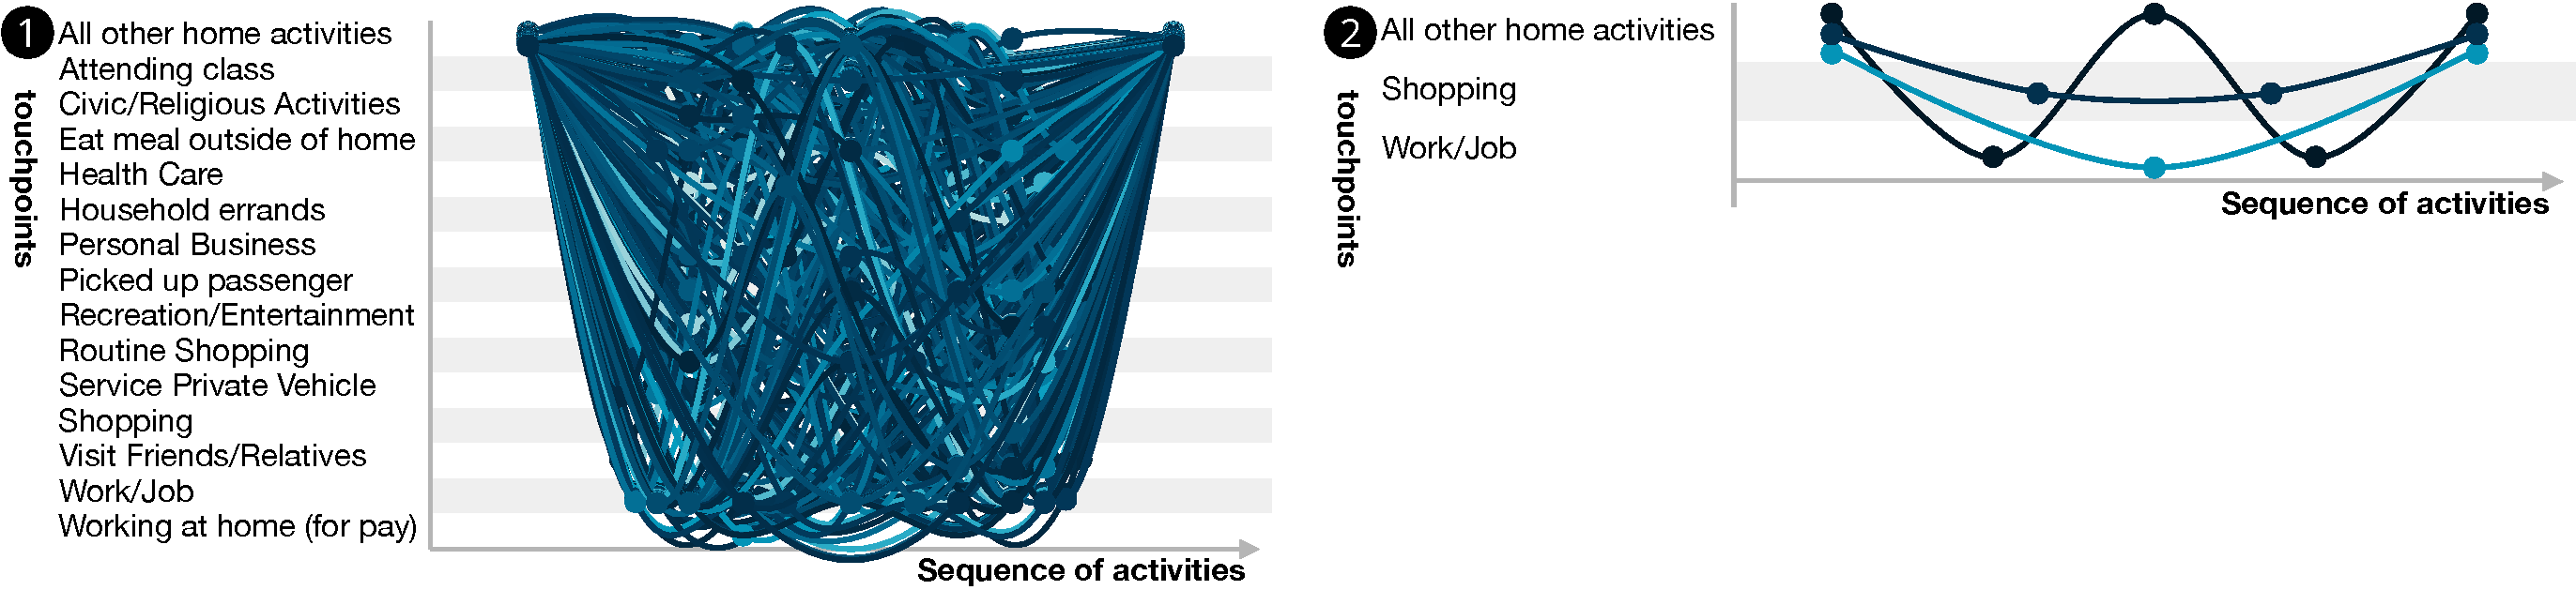
\includegraphics[width=1\columnwidth]{05_schema/intro2.pdf}
\caption{\ding{202} Less than 0.01\% of the entire dataset on a CJM, and \ding{203}, a  summary of the dataset using 3 representatives.}
\label{representativejourney}
\end{figure}

Fig.~\ref{representativejourney} shows CJMs derived from a real dataset\footnote{http://www.cmap.illinois.gov/data/transportation/travel-survey
}. In this dataset, a journey is all the activities that are performed by a citizen throughout the day. For instance being at home, attending class and going back home is one of the potential journeys. As can be seen in \ding{202} of Fig.~{\ref{representativejourney}}, displaying such actual journeys on the CJM without preprocessing the data results in an overwhelming chart. It becomes clear that when a company deals with very large numbers of actual journeys, it is necessary to reduce the complexity and to look at these journeys at a higher level of abstraction. Specifically, representative journeys address this issue, \cite{bernard2019genetic}, by summarizing the dataset (using three journeys visible in \ding{203} of Fig.~\ref{representativejourney}). 

\begin{figure}[H]
\centering
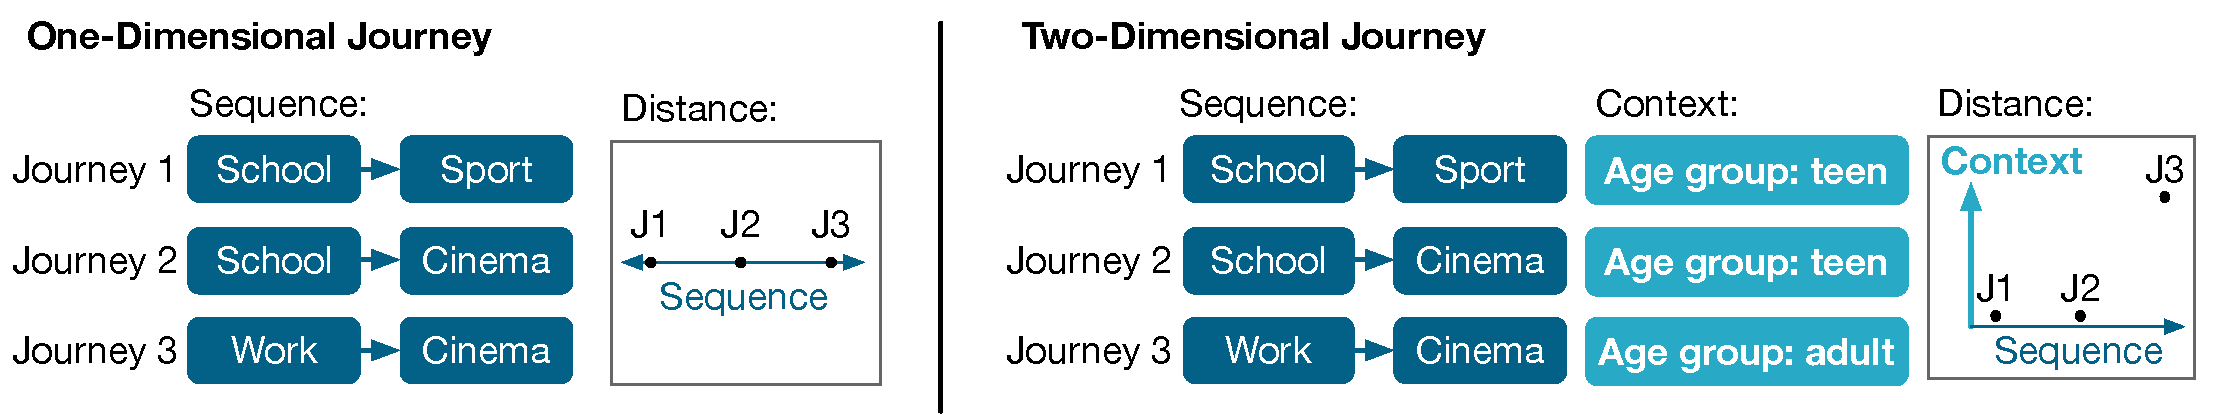
\includegraphics[width=1\columnwidth]{05_schema/context1.pdf}
\caption{Measuring the distance among three journeys with and without the context.}
\label{context1}
\end{figure}

The existing solutions to summarize collections of journeys \cite{gabadinho2009summarizing,bernard2019genetic} consider only the sequence of touchpoints when measuring the distance between journeys. Fig.~\ref{context1} illustrates the process with 3 short journeys. Using a basic distance measure between sequences (e.g., edit-distance), we cannot say which one of `Journey 1' or `Journey 3' is closer to `Journey 2' (left-part of Fig.~\ref{context1}). We suggest that demographics and other contextual information might be equally important to measure the distance between journeys. Hence, in this paper, we propose to integrate such information when mining journeys. The right-part of Fig.~\ref{context1} shows that when we also consider the age group, it becomes clearer that the closest journey to `Journey 2' is `Journey 1'.

{\it We propose an algorithm summarizing a customer experience using both the sequence of activities as well as the contextual information.} Our genetic approach uses only three intuitive parameters: 1) the approximate number of representative journey to use, 2) the weight of the sequence of activities, and 3) the weight of the contextual data. We demonstrate in the evaluation section that our approach outperforms existing techniques. Finally, we highlight the impact of the three parameters using a real dataset and illustrate the results with CJMs. 

The paper is organized as follows. Section 2 clarifies the customer journey discovery activity. In Section 3, we outline of existing techniques. Section 4 depicts our genetic algorithm. In Section 5, we evaluate the results using internal and external evaluation metrics. Section 6 illustrates CJMs produced by our algorithm. Finally, Section 7 concludes the paper. 


\section{Customer Journey Discovery}
The goal of a customer journey discovery algorithm is to find a reasonable amount of representative journeys that well summarizes actual journeys. 

\textbf{Definition 1} (Touchpoint): a touchpoint is an interaction between a customer and a company's products or services \cite{bernard2017cjm}. {`Sharing on social network' or `ordering a product on the website' are two typical examples of touchpoints in a retail context. We define $t$ as the touchpoint, and $T$ the finite set of all touchpoints. The touchpoints are visible in the y-axis of the CJMs (Fig. \ref{representativejourney}).

\textbf{Definition 2} (Actual Journey): An actual journey $J_a$ is a sequence of touchpoints observed from customers. For instance, $J_a$ = \{$\langle$`Visiting the shop', `Testing the product', `Sharing on social network'$\rangle$}\} is a journey with three touchpoints. For the sake of brevity, we replace the touchpoints with alphabetical characters so that $J$ becomes $\langle$ABC$\rangle$. The order in which the activities are executed is represented by the x-axis of the CJMs visible in Fig. \ref{representativejourney}.

\textbf{Definition 3} (Representative Journey): A representative journey, $J_{r}$, is a journey that summarizes a subset of actual journeys. The left-part of Fig. \ref{representativejourney} shows how a CJM would look like when we display actual journeys, while the right-part uses representative journeys. Clearly, as can be seen in Fig. \ref{representativejourney}, the use of  representative journeys increases the readability of the CJM. 

\textbf{Definition 4} (Event Logs): Let $J_{\mathcal{A}}$ be an event log, which we define as the collection of all actual journeys observed by customers. 

\textbf{Definition 5} (Customer Journey Map): A customer journey map summarizes customer journeys through the use of representative journeys. Let a customer journey map $J_{\mathcal{R}}$ be the set of all the $J_{r}$s summarizing $J_{\mathcal{A}}$. Let $k_{\mathcal{R}}$ denote the number of journeys in a map (i.e., $|J_{\mathcal{R}}|$). Typically, the part \ding{203} of Fig.~\ref{representativejourney} is a CJM, $J_{\mathcal{R}}$, containing three representative journeys summarizing an event logs.

{\it The customer journey discovery activity can be defined as a function that maps all members of $J_{\mathcal{A}}$ to a member of $J_{\mathcal{R}}$;} i.e., that maps all the actual journeys to representative journeys ultimately displayed on a CJM. Discovering customer journeys from event logs is an unsupervised clustering task that entails interesting challenges. First, there is no evidence in the literature that deals with the ideal number of representative journeys to use. When the goal is to have a general overview about dataset, it seems reasonable to display only few journeys so the CJM is readable. However, discovering few dozens representative journeys might also be a relevant choice if the goal is to catch complex and less generic patterns. Finally, the sequence that best summarizes its assigned actual journeys needs to be found. It might be the case that an ideal representative journey was never observed but well summarizes the actual journeys. This phenomena was observed by Gabadinho et al., and illustrated as follows: ``We could imagine synthetic -- not observed -- typical sequences, in the same way as the mean of a series of numbers that is generally not an observable individual value.'' \cite{gabadinho2009extracting}. Before presenting our solution, the next section describes related work.

\section{Related Work}
Our work is close to the summarization of categorical sequences used in social sciences. In \cite{gabadinho2009summarizing,gabadinho2009extracting}, Gabadinho et al. propose summarizing a list of observed sequences (i.e., actual journeys) using a representative (i.e., a representative journey). They define a representative set as {\it``a set of non-redundant `typical' sequences that largely, though not necessarily exhaustively, cover the spectrum of observed sequences''} \cite{gabadinho2009summarizing}. We argue that it matches our definition of a representative sequence summarizing a set of sequences. The authors propose multiple ways to select a representative. The {\it `frequency'} (1), where the most frequent event is used as the representative. The {\it `neighborhood density'} (2), which consider the representative as the sequence with the most neighborhood in a defined diameter. The {\it `centrality'} (3): the representative {-- or medoid --} can be found using the centrality. {Being the most central object,} the representative is the sequence with the minimal sum of distances to all other sequences. Finally, the {\it `sequence likelihood'} (4): the sequence likelihood of a sequence derived from the first-order Markov model can also be used to find the representative. 

Because it starts from data in order to produce conceptual models, process mining is another discipline closely related to the topic of customer journey discovery. The link between customer journey maps and process mining was highlighted in \cite{bernard2017cjm}. However, business process models and CJMs are not built for the same purpose. While a business process model captures how a process was or should be orchestrated, a CJM is built for the purpose of better understanding what customers have experienced. Gartner highlighted that CJMs are used to supplement but not to replace BPMs \cite{Gartner2015}.

In \cite{bernard2017cjmEX}, we propose CJM-ex, a web-based tool to navigate CJMs. It uses a hierarchical structure that allows drilling-down in customer journeys. In \cite{bernard2017Markov}, it was shown that customer journey maps can be discovered using Markov model. In \cite{bernard2019genetic}, we suggested a genetic approach to discover representative journeys that uses only the sequence of touchpoints to measure the distance between journeys. Hence, this current work can be seen as an extension of \cite{bernard2019genetic} to allow taking both the sequence of touchpoints and the contextual information into account when build CJMs. 


\section{Genetic Algorithm for CJM Discovery}

%{Our work is inspired by the genetic approaches proposed in} \cite{buijs2012genetic,vazquez2015prodigen,de2005genetic} {to discover business process models from event logs. However, we tailored it towards CJMs by introducing specific evaluation metrics suited for them.} Fig.~\ref{fig:process} depicts the main phases: (1) a preprocessing phase, (2) generating the initial population, (3) assigning each actual journey to its closest representative, (4) evaluating the quality of the CJMs, (5) the stopping criterion evaluation, and (6) creating new CJMs by applying some genetic operations.

\begin{figure}[H]
\centering
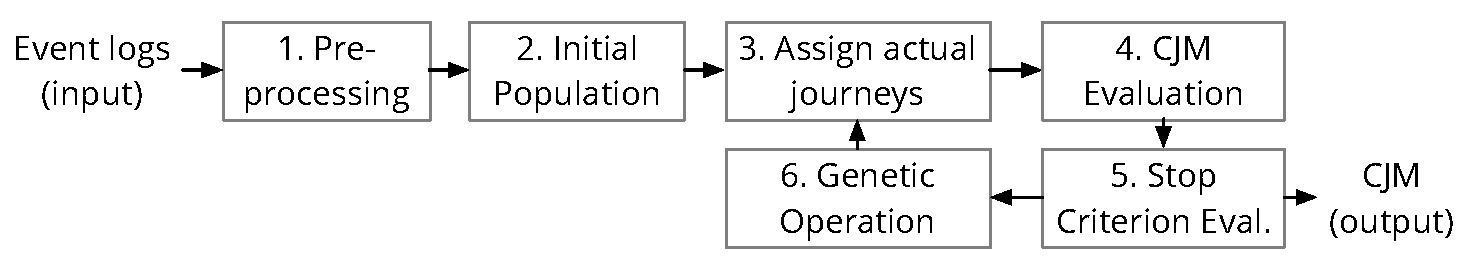
\includegraphics[width=0.8\columnwidth]{05_schema/process.pdf}
  \caption{Overview of the genetic algorithm to discover CJMs}
  \label{fig:process}
\end{figure}


As an introduction, Fig.~\ref{fig:process} provides intuition on how the genetic algorithm builds a CJM. A set of actual journeys, $J_{a}$, is provided to the algorithm. Then, during  {\it Generation 1}, we build $p$ number of $J_{\mathcal{R}}$, where {\it $p$ is the population size}; i.e., the number of CJMs that will be evaluated after each generation. In Fig.~\ref{fig:intuition2}, $p$ is 3. Each $J_{\mathcal{R}}$ is evaluated and we keep the $e$ best $J_{\mathcal{R}}$s, called the {\it elite set} while we discard the other ($p-e$) $J_{\mathcal{R}}$s. Then, we move to {\it Generation 2}, where we keep an untouched version of the $e$ number of $J_{\mathcal{R}}$s in the elite set. In Fig.~\ref{fig:intuition2}, $e$ is set to 1. For instance, $J_{\mathcal{R}2}$ was kept in Generation 2 because it has the best average quality in Generation 1, i.e., $J_{\mathcal{R}2}$ is intact in Generation 2. We then apply some transformation (to be discussed next) to generate ($p-e$) new $J_{\mathcal{R}}$s that will, in turn, be evaluated. In our case, we generate $J_{\mathcal{R}4}$ and $J_{\mathcal{R}5}$. We recursively transform and evaluate the $p$ number of $J_{\mathcal{R}}$s until a stopping criterion is met. Once a stopping criterion is met, we return the best $J_{\mathcal{R}}$ ($J_{\mathcal{R}7}$ in Fig.~\ref{fig:intuition2}). { \it The best $J_{\mathcal{R}}$ can be interpreted as the best set of representative journeys, $J_r$, representing a set of journeys from $J_{\mathcal{A}}$ that have been found given a certain evaluation criterion.} The next section describes how we generate the initial population, what various types of operations we apply on each $J_{\mathcal{R}}$ to transform them, and how we evaluate each one of them given a set of journeys in $J_{\mathcal{A}}$. 

\begin{figure}
\centering
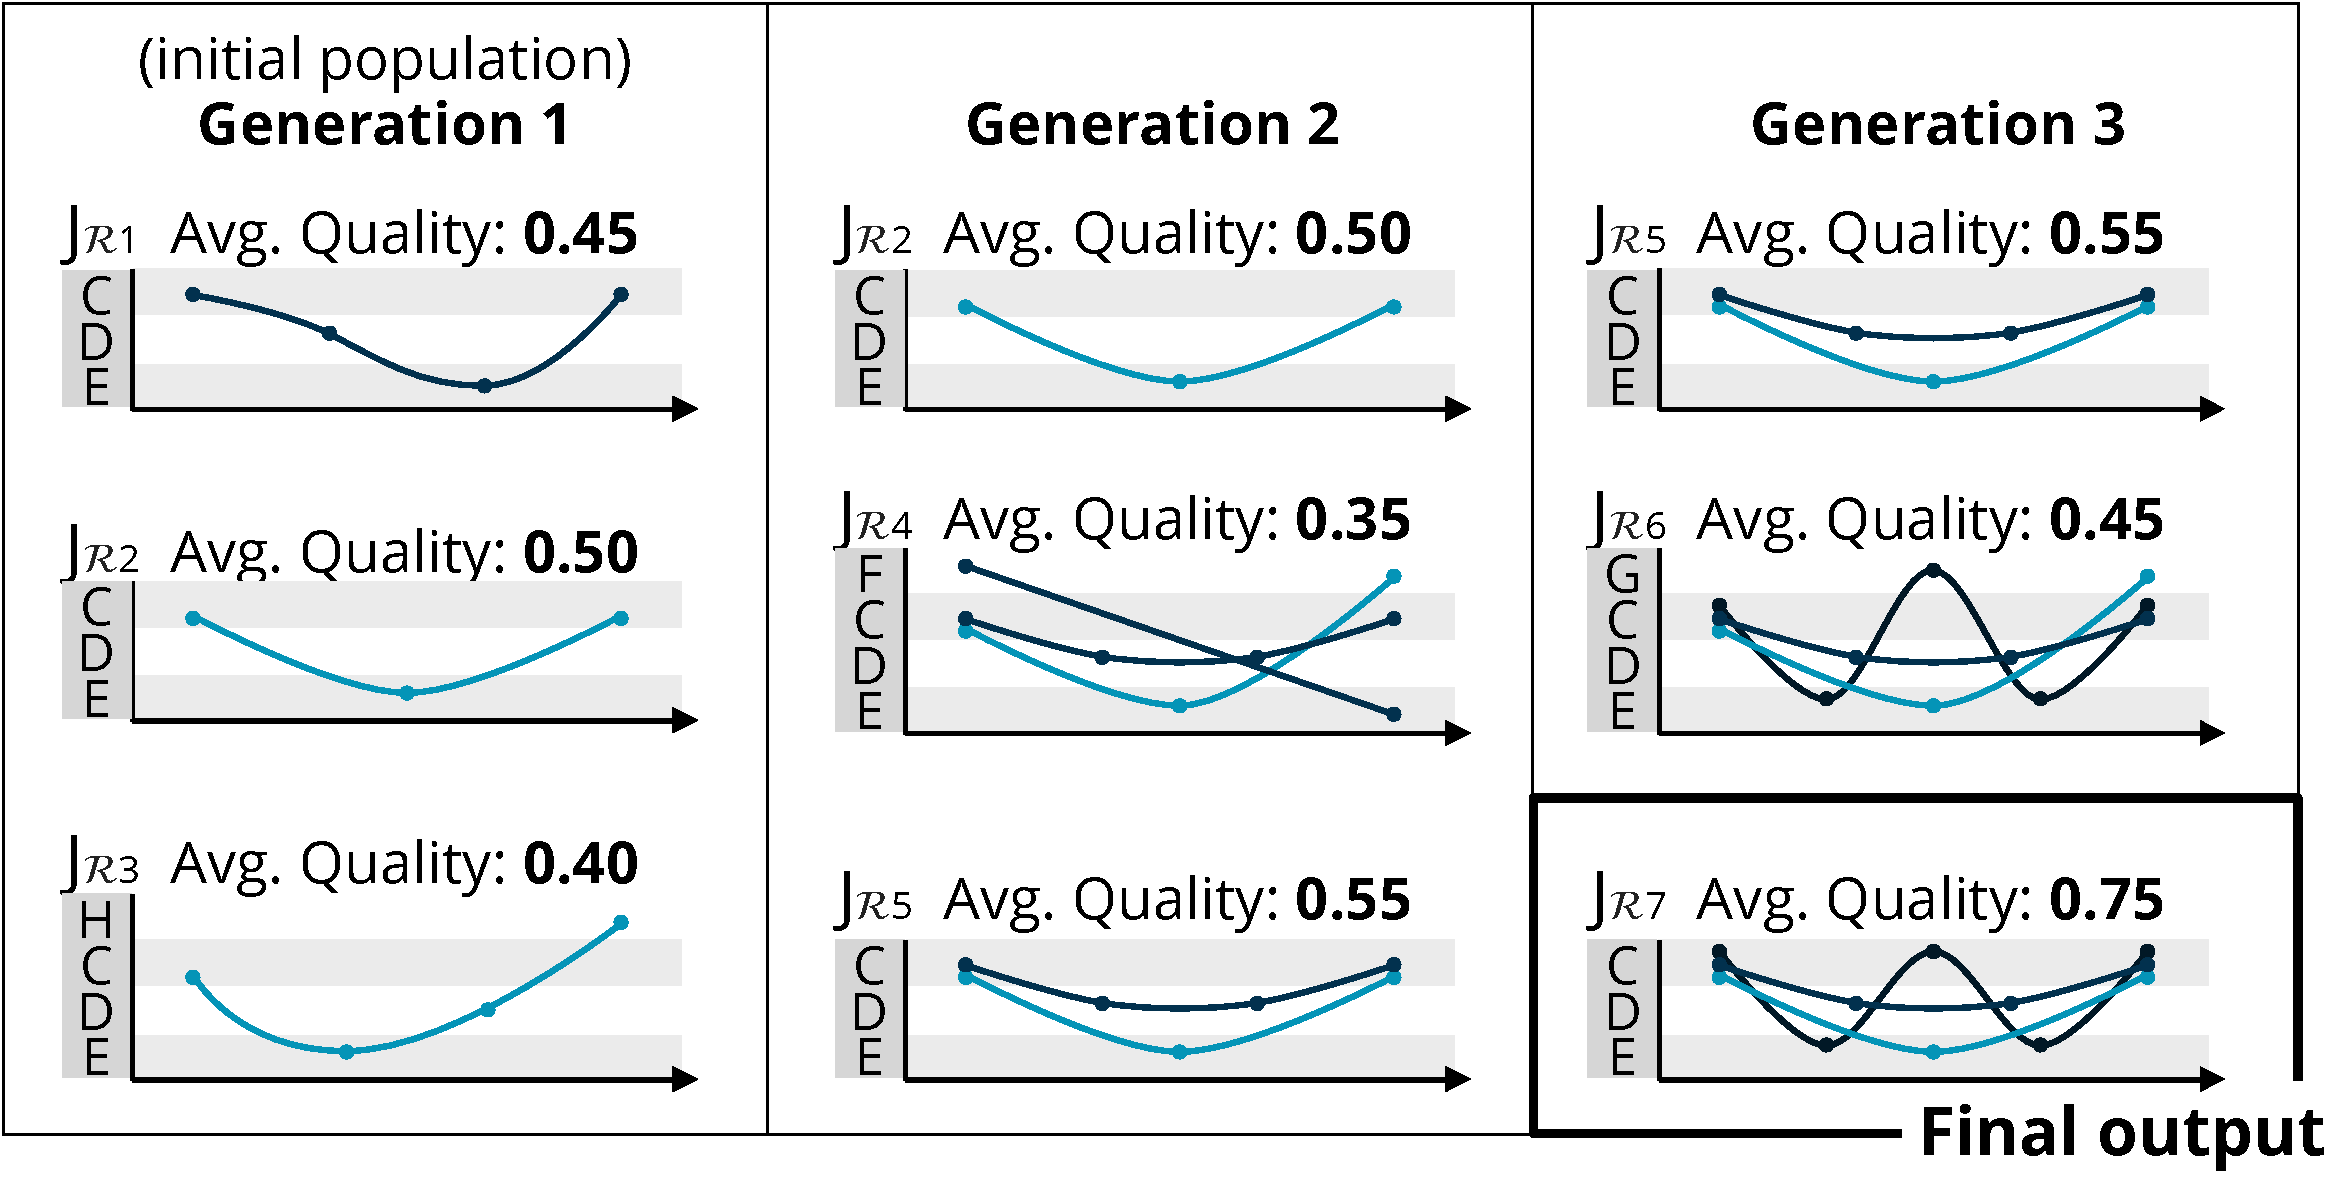
\includegraphics[width=0.7\columnwidth]{05_schema/intuition2.pdf}
  \caption{Illustration of the genetic process to discover the best CJM}
  \label{fig:intuition2}
\end{figure}

\subsection{Preprocessing} \label{preprocessing}
To gain in efficiency, we make the assumption that $J_{\mathcal{R}}$ will be close to the frequent patterns observed in $J_{a}$. Let $Top_{\ell_n}$ be the $n$ most occurring patterns of length $\ell$ and $Top_n \supseteq Top_{\ell_{[2,m]}}$ be the superset of all the most occurring patterns of lengths $2$ to $m$.  $Top_n$ is used later to form the initial population of $J_{\mathcal{R}}$ (described in Section \ref{chap:initial-population}), and to add a random journey to $J_{\mathcal{R}}$. Using $Top_n$ we avoid generating journeys by picking a random number of touchpoints from $T$. According to our experiments, using $Top_n$ reduces the execution time by two to get an output $J_{\mathcal{R}}$ of the same average quality.

\subsection{Initial Population}
\label{chap:initial-population}
The initial population is generated by adding a sequence randomly picked from $Top_n$ {(defined in Sect. \ref{preprocessing})}. In our running example, depicted in Fig.~\ref{fig:intuition2}, the initial population is visible in column `generation 1'. In Fig.~\ref{fig:intuition2}, the population size is 3. In our experiments, we set the population size to 100. 

\subsection{Assign Actual Journeys}
The quality of a representative journey can only be measured when knowing which actual journeys it represents. Hence, a first step toward evaluating the quality of $J_{\mathcal{R}}$ is to assign each journey $J_a \in J_{\mathcal{A}}$ to its closest journey in $J_r \in J_{\mathcal{R}}$. To characterize the closeness between $J_a$ and $J_r$, we use the Levenshtein distance borrowed from \cite{levenshtein1966binary}. It is a metric particularly well-suited to measure the distance between sequences. The Levenshtein distance counts the number of edit operations that are necessary to transform one sequence into another one. There are three types of operations: deletions, insertions, and substitutions. For instance, the distance between {$\langle \textsc{abc} \rangle$} and {$\langle \textsc{acce} \rangle$} is 2 since one substitution and one insertion are required to match them. We define the closest representative as the one having the smallest Levenshtein distance with the actual journeys. Note that if a tie occurs between multiple best representatives, we assign the $J_a$ to the $J_r$ having the smallest amount of actual journeys already assigned to it. Once each actual journey has been assigned to its closest representative, we can evaluate $J_{\mathcal{R}}$ using the criteria described in the next section. 
 

\subsection{CJM Evaluation Criteria}
\label{chapter:cjm-evaluation-criteria}

This section introduces the evaluation criteria used to determine the quality of each $J_{\mathcal{R}}$, namely, (1) the fitness, (2) the number of representatives, (3) the contextual distance, and (4) the average quality.  

\subsubsection{Fitness.} The fitness measures the distance between each sequence of activities $J_{a}$ and its closest representative $J_{\mathcal{R}}$ using the Levenshtein distance \cite{levenshtein1966binary}. 
\begin{equation}
\footnotesize
    Fitness(J_{a}, J_{\mathcal{R}}) =  
    1-\frac
      {\sum_{i=1}^{|J_{a}|}min_{j=1}^{|J_{\mathcal{R}}|}({Levenshtein(\mathbf{\sigma_{\mathcal{A}_i}}}; \mathbf{\sigma_{\mathcal{R}_j}}))}
      {\sum_{i=1}^{|J_{a}|}{Length(\sigma_{\mathcal{A}_i})}}
\end{equation}
where 
\begin{conditions*}
 \mathbf{\sigma_{\mathcal{A}_i}} &  i\textsuperscript{th} actual sequence  observed in event logs \\
 \mathbf{\sigma_{\mathcal{R}_j}} &  j\textsuperscript{th} representative contained in $J_{\mathcal{R}}$ \\
 Length(x)  &  Length of the sequence of activity $x$
\end{conditions*} 

A fitness of 1 means that the representative journey perfectly catches the behavior of the actual journeys assigned to it. In contrast, a fitness close to 0 implies that many edit operations are necessary to match the sequences.

\subsubsection{Number of Representatives.} An event log can contain several hundreds or thousands of unique actual journeys. Hence, we maximize the fitness without trying to keep a low $k_{\mathcal{R}}$, the CJM will become unreadable because too many representative journeys will be displayed in it. In other words, $J_{\mathcal{R}}$ overfits. Hence, the goal is to find a $k_{\mathcal{R}}$ that offers a good compromise between underfitting and overfitting. Finding the optimal number of clusters is a recurrent challenge when clustering data. We propose integrating traditional ways of determining the optimal number of clusters, such as the Bayesian information criterion \cite{schwarz1978estimating},  or the Calinski-Harabasz index \cite{calinski1974dendrite}. The idea is to evaluate a range of solutions (e.g., from 2 to 10 journeys) and to keep the best solution. Let $k_{h}$ be the optimal number of clusters returned by one of the techniques mentioned above. By integrating $k_{h}$ into the evaluation, we can guide the solution toward a $k_{\mathcal{R}}$ that is statistically relevant. To evaluate the quality, we measure the distance between $k_{\mathcal{R}}$ and $k_{h}$. To do this, we propose the following distribution function:

\begin{equation}
\footnotesize
    Number Of Representatives({k_{\mathcal{R}}}, {k_{h}}, {x_0}) = \frac{1}{1 + (\frac{|k_{\mathcal{R}}-k_{h}|}{x_0})^{2} } 
\end{equation}

where 
\begin{conditions*}
 $${k_{\mathcal{R}}}$$  &  Number of $J_r$ journeys on $J_{\mathcal{R}}$ (i.e., $|J_{\mathcal{R}}|$)\\
 $${k_{h}}$$  &  Optimal number of journeys (e.g., using the Calinski-Harabasz index)\\
 $${x_0}$$  &  x value of the midpoint \\
\end{conditions*} 

The parameter $x_0$ determines where the midpoint of the curve is. Concretely, if $x_0=5$, $k_{\mathcal{R}}=11$ will result in a quality of 0.5 because the absolute distance from $k_{h}$ is 5. We set $x_{0}=5$ for all our experiments. Because the number of representatives is not the only criteria to assess the quality of a CJM, the final CJM might contain more or less journeys if it increases the average quality.

%to be improved !
\label{contextual-distance}
\subsubsection{Contextual Distance.} The contextual distance allows us to consider the set of contextual data $C$ when grouping similar journeys. The more distant the set of contextual data is between $J_a$ that are represented by distinct $J_r$, the better the quality is. To measure the distance, we first build a value frequency table which count all the values per representatives (${v_i}$ is the value frequency counter for $J_{r_i})$. Then, for each pair of clusters, we calculate the cosine similarity, which is defined as:

\begin{equation}
\footnotesize
    ContextualDistance({v_{1}}, {v_{2}}) = \frac{v_{1} \cdot v_{2}}{||v_{1} ||\cdot||v_{2}||} 
\end{equation}

Finally, the cosine distances are averaged to get the overall contextual distance. A short overall distance indicates that the contextual data of $J_a$ that are assigned to distinct $J_r$ are similar. In other words, the contextual data does not help in classifying $J_a$ between several $J_r$. 

\subsubsection{Average Quality. } We assign weights to the fitness, the number of representatives, and the contextual distances qualities to adjust their relative importance. Then, we get the overall quality by averaging the weighted qualities using the arithmetic mean. 

\subsection{Stopping Criterion}
{Once we assess the quality of generated CJMs, we check if a stopping criterion is met.} There are three ways we can use to stop the algorithm taken from \cite{buijs2012genetic,de2005genetic}. (1) The algorithm could stop after a certain number of generations. (2) One could stop the algorithm when a certain number of generations have been created without improving the average quality. (3) We could stop the algorithm when a certain quality threshold is reached for one of the evaluation criteria. Because it is difficult to predict the quality level that can be reached, we believe that stopping the algorithm using a threshold is not advisable. For this reason, we used a combination of approaches 1 and 2 for our experiments. Once the stopping criteria have been evaluated, there are two outcomes. Either one of the criteria is met and the algorithm stops, returning the best $J_{\mathcal{R}}$, or, {we generate new candidates} by recursively calling a function that generates the next population, described in the next section.

\subsection{Genetic Operations}
Once all the CJMs have been evaluated, we rank them by their average quality and copy a fraction (i.e., $e$) of the best ones in {$elite$}. In Fig.~\ref{fig:intuition2}, the elite size is 1. In our experiments, we set the elite size to 5. Because we keep an untouched version of the $e$ number of $J_{\mathcal{R}}$s, we make sure that the overall quality will only increase or stay steady. Then, we generate $(p-e)$ new $J_{\mathcal{R}}$s as follows. {\it (1) Add a random journey (mutation):} A sequence is randomly picked from $Top_n$ and added to $J_{\mathcal{R}}$. {\it (2) Add an existing journey (crossover):} An existing representative journey is randomly picked from the elite population and added to $J_{\mathcal{R}}$. {\it (3) Delete a journey (mutation):} A random journey is removed from $J_{\mathcal{R}}$. Nothing happens if $J_{\mathcal{R}}$ contains only one journey. {\it (4) Add a touchpoint (mutation):} A touchpoint from $T$ is added to one of the journeys from $J_{\mathcal{R}}$ at a random position. {\it (5) Delete a touchpoint (mutation):} A touchpoint is removed from $J_{\mathcal{R}}$ unless removing this touchpoint would result in an empty set of touchpoints. 

In Fig.~\ref{fig:intuition2}, $J_{\mathcal{R}5}$ have been produced by taking $J_{\mathcal{R}2}$ and adding a journey picked from $Top_n$ (defined in Sect. \ref{preprocessing}). As described in Fig.~\ref{fig:process}, once new $J_{\mathcal{R}}$s have been created, we go back to the evaluation phase where the new $J_{\mathcal{R}}$s are evaluated until one stopping criterion is met. Once such a criterion is met, we return the best $J_{\mathcal{R}}$s of the last generation (e.g., $J_{\mathcal{R}7}$ in Fig.~\ref{fig:intuition2}) and the algorithm stops.

We loop over each of these 5 types of transformations three times. Each time, the probability of applying the transformation is 10\%, which means that more than one transformation is applied. It also means that the same transformation might be applied up to three times (with a probability of 0.1\%). At the very least, one transformation has to be applied. If it is not the case, we loop over each transformation three times again until at least a transformation is applied.

\section{Evaluation Using Synthetic Datasets}
In order to evaluate the quality of our approach to return the best set of representative journeys in $J_{\mathcal{R}}$, we evaluate the results using a collection of synthetic customer journeys that includes some contextual data. We first describe how we generated the dataset. Then, using this synthetic dataset, we evaluate and compare our algorithm with state-of-the-art techniques to summarize sequences of categorical data. 

\subsection{Datasets}


\begin{wrapfigure}{l}{0.45\textwidth}
  \begin{center}
    \raisebox{0pt}[\dimexpr\height-3\baselineskip\relax]{\
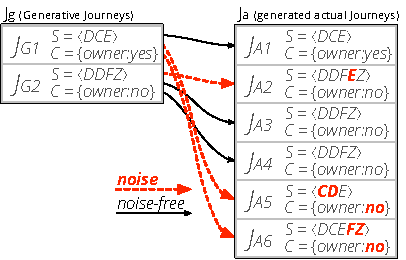
\includegraphics[width=0.42\columnwidth]{05_schema/dataset.pdf}
    }
  \end{center}
  \vspace{-5pt}
  \caption{Dataset with 50\% of noise.}
  \label{fig:dataset}
\end{wrapfigure} 


To evaluate the results of our algorithm, we produced several event logs that simulate journeys. Generating the event logs ourselves means that we know the ground truth represented by the generative journeys and therefore our task would be to recover these journeys from a set of actual ones we produce. A generative journey is a known sequence of activities with a known set of characteristics from which we generate the event logs. If we were to use only these generative journeys to generate 1,000 thousand journeys, we would obtain only {$k_{\mathcal{G}}$ distinct journeys. From a business point of view, this would describe an ideal situation where each group of customers behaves in an homogeneous way. However, we know that this is not the case. A more realistic situation would depict a scenario where each group of customers can be described by a representative sequence of activities, but the actual journeys within the group can deviate from the representative one. To produce more realistic data, we inject noise for a fraction of the journeys. For instance, if the noise level is set to 50\%, $J_a = J_g$ is true for half of the data. Fig.~\ref{fig:dataset} illustrates how six journeys are generated from two generative journeys. If we assume that the noise level is defined to be 50\%, three actual journeys in the events logs deviate from the original generative journeys. The goal of our experiments is to retrieve the set of generative journeys, as representatives, from the produced actual journeys. The 40 generated datasets as well as details on how we produced them are made publicly available\footnote{\url{http://customer-journey.unil.ch/datasets/}}.

\subsection{Metrics}
To evaluate and compare the quality of representative journeys, we use both external and internal evaluation metrics. On the one hand, the external ones evaluate the results relative to the ground truth, i.e., from the generative journeys. On the other hand, the internal evaluation uses cluster analysis techniques to assess the results. The aim is to account for the fact that the ground truth might not be the optimal solution. Indeed, adding random noise might change the optimal solution. This section introduces these metrics. For the internal evaluation metrics, we borrowed metrics from \cite{gabadinho2009extracting}.


\subsubsection{External Evaluation - Distance in Number of Journeys.} This metric measures the distance between the number of generative journeys and the number of representative journeys returned by the algorithm. We propose the following metric:
\begin{equation}
\footnotesize
    NbJourneysDistance({k_{\mathcal{G}}}, {k_{\mathcal{R}}}) = abs({k_{\mathcal{G}}} - {k_{\mathcal{R}}}) 
\end{equation}

\subsubsection{External Evaluation - Jaccard Distance.} To evaluate the distance between the sequences of activities from the generative journeys ($\sigma_{\mathcal{G}}$) and the discovered representative journeys ($\sigma_{\mathcal{R}}$), we propose to use the Jaccard Distance where a score of 1 indicates a perfect match between the set of sequences from the generative journeys and the representative ones. 
\begin{equation}
\footnotesize
    JaccardDistance(\mathbf{\sigma_{\mathcal{R}}}, \sigma_{\mathcal{G}}) = 1 - \frac{|\mathbf{\sigma_{\mathcal{R}} \cap \sigma_{\mathcal{G}}}|}{|\mathbf{\sigma_{\mathcal{R}} \cup \sigma_{\mathcal{G}}}|}
\end{equation}

\subsubsection{Internal Evaluation - Mean distance \cite{gabadinho2009extracting}.} The mean distance $i$ returns the average distance between the representative sequence $i$ and the sequence of actual journeys that have been assigned to $i$. If the mean distance $i$ is 0, then the representative journey $i$ perfectly matches the underlying actual journeys.   
\begin{equation}
\footnotesize
    MeanDistanceScore_i = \frac{\sum^{k_i}_{j=1}{D(S_{i}}, S_{ij})}{k_i}
\end{equation}
where 
\begin{conditions*}
  D(x_1,x_2)  &  Levenshtein distance between two sequences  \\
  k_i & Number of actual journeys assigned to the representative journey $i$  \\
  S_i & Representative sequence $i$  \\
  S_{ij} & Sequence of actual journeys $j$ assigned to $i$  \\
\end{conditions*} 

\subsubsection{Internal Evaluation - Coverage \cite{gabadinho2009extracting}.} The coverage indicates the proportion of actual journeys that are within the neighborhood $n$ of a representative.   
\begin{equation}
\footnotesize
    Coverage_i = \frac{\sum^{k_i}_{j=1}{(D(S_{i}}, S_{ij}) < n)}{k_i}
\end{equation}
where 
\begin{conditions*}
  D(x_1,x_2)  &  Levenshtein distance between two sequences  \\
  k_i & Number of actual journeys assigned to the representative journey $i$  \\
  S_i & Representative sequence $i$  \\
  S_{ij} & Sequence of actual journeys $j$ assigned to $i$  \\
\end{conditions*} 

\subsubsection{Internal Evaluation - Distance gain \cite{gabadinho2009extracting}.} The distance gain measures the gain in using a representative journey instead of the true center of the set (i.e., the medoid of the whole dataset). In other words, it measures the gain obtained in using multiple representative journeys instead of a single one.   
\begin{equation}
\footnotesize
    DistGain_i = \frac{\sum^{k_i}_{j=1}{D(C(\sigma_{\mathcal{A}})}, S_{ij})-\sum^{k_i}_{j=1}{D(S_{i}}, S_{ij})}{\sum^{k_i}_{j=1}{D(C(\sigma_{\mathcal{A}})}, S_{ij})} 
\end{equation}
where 
\begin{conditions*}
  D(x_1,x_2)  &  Levenshtein distance between two sequences  \\
  k_i & Number of actual journeys assigned to the representative journey $i$  \\
  S_i & Representative sequence $i$  \\
  S_{ij} & Sequence of actual journeys $j$ assigned to $i$  \\
  C(x)  &  True center of the set  \\
\end{conditions*} 

\begin{figure}[t]
\centering
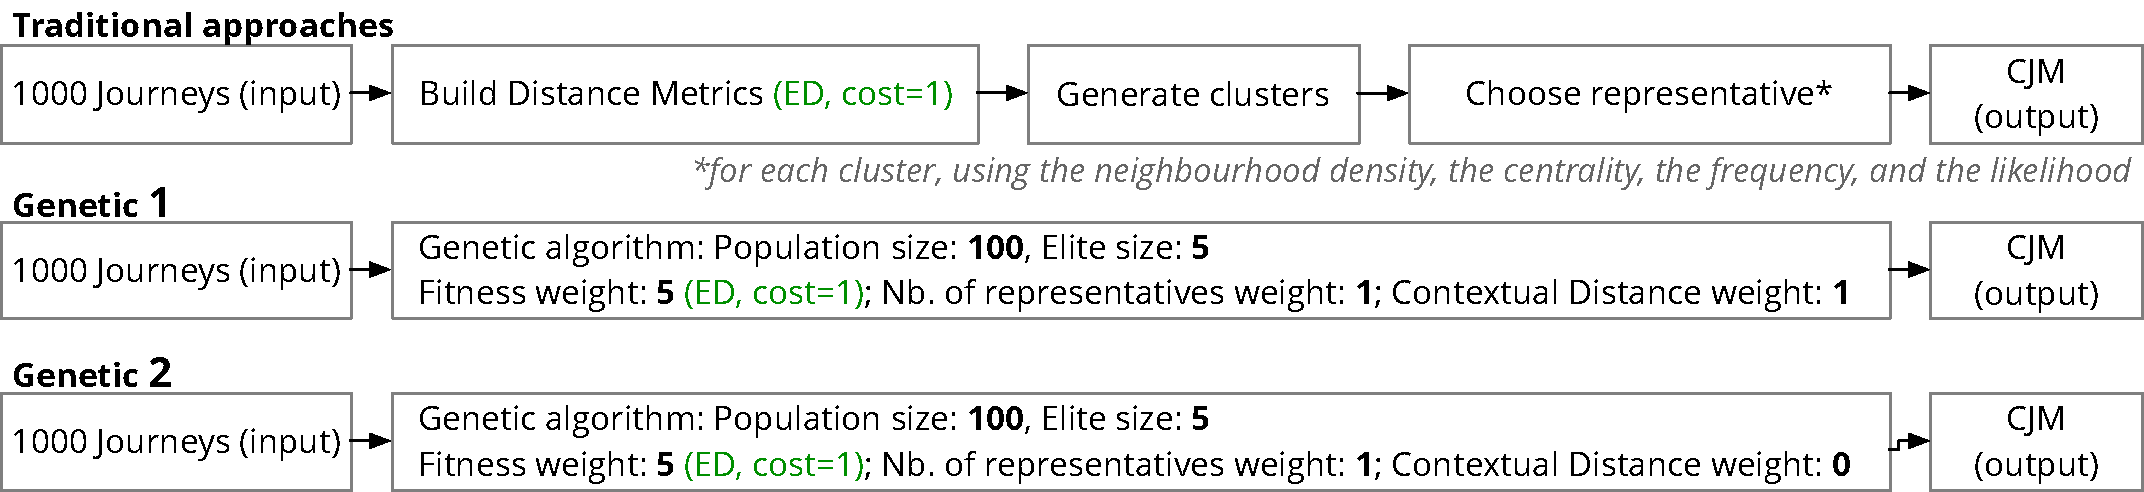
\includegraphics[width=1\columnwidth]{05_schema/settings2.pdf}
\caption{Approach used to evaluate our clustering algorithm from traditional approaches.}
\label{fig:approach}
\end{figure}

\subsection{Settings}
We evaluate two settings of our genetic algorithm against traditional approaches. The traditional approaches are state-of-the-art techniques that are used to cluster and summarize sets of sequential and categorical data. Fig.~\ref{fig:approach} depicts the approach at a high-level. As can be seen, with traditional approaches, we first build a distance metric. We use the edit distance with a constant cost operation set to 1. Once the distance matrix is built, we create $k$ clusters. Because we do not know the number of representative journeys to be found, we test using from 2 to 12 clusters and use the squared Calinski-Harabasz index described in \cite{calinski1974dendrite} to return the most statistically relevant. Then, we return the best representatives of each cluster using the neighborhood density, the centrality, the frequency, or the likelihood {using the package Traminer available in R \cite{gabadinho2013searching}}. These techniques do not use the contextual data. Hence, to allow for a fair comparison, we compare these techniques with a version of our genetic algorithm that does not use contextual data and which was presented in \cite{bernard2019genetic}. {We call this version {$Genetic_1$}.} We also test our genetic algorithm with a version that considers the contextual data, called $Genetic_2$. Note that both the traditional and genetic approaches use the same techniques to find $k_{h}$ and the distance is measured using the edit distance with a constant cost operation set to 1. Due to the non-deterministic nature of the genetic algorithm, we run it ten times for each setting.

\subsection{Results}
Fig.~\ref{fig:results} shows the external evaluation metrics. It can be seen that the best solution is the $Genetic_2$, highlighting that considering the contextual information when grouping journeys improves the quality. Next, the best solution that does not use contextual data is $Genetic_1$ proposed in \cite{bernard2019genetic}. 

\begin{figure}[H]
\centering
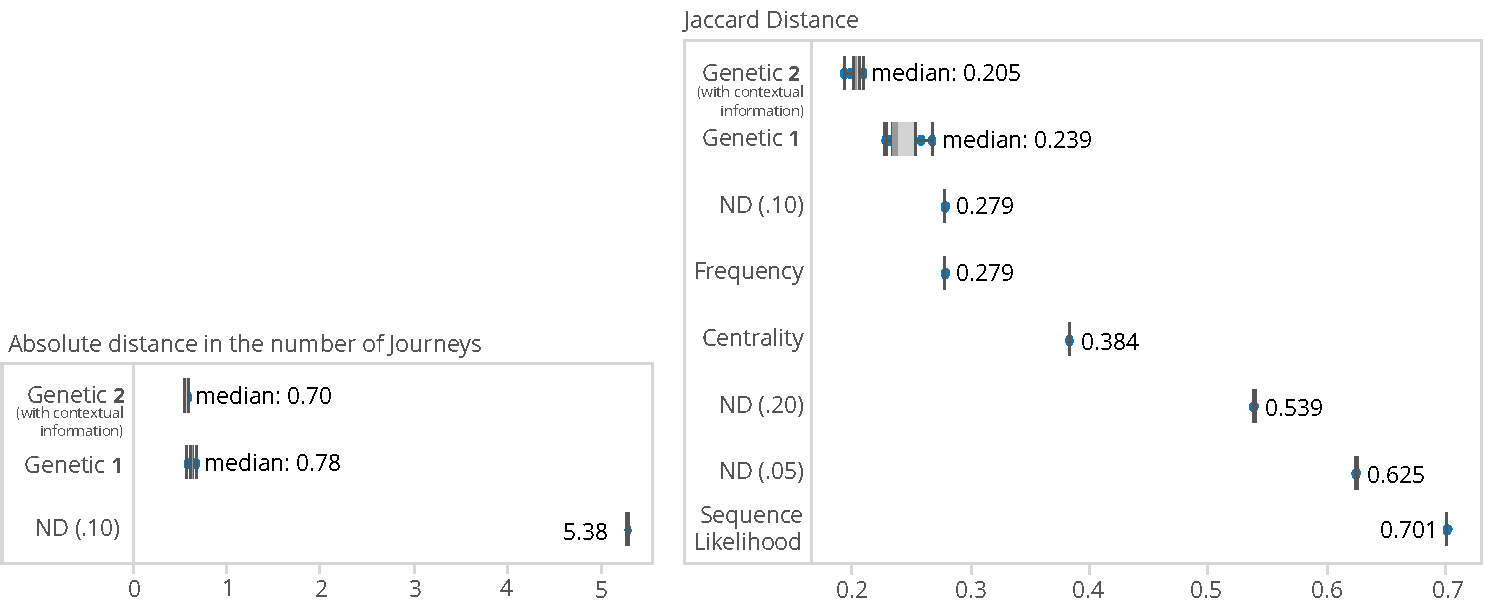
\includegraphics[width=0.92\columnwidth]{05_schema/results_len.pdf}
  \caption{External evaluation. The genetic algorithm that uses the contextual information (i.e., $Genetic_2$) performs best.}
  \label{fig:results}
\end{figure}

The internal evaluation of Fig.~\ref{fig:eval_internal} shows that not only does the genetic algorithm outperform the traditional approaches, it also proposes a better solution than the ground truth. This can be explained by the fact that when we inject noise, we potentially change the optimal solution.  



\begin{figure}[H]
\centering
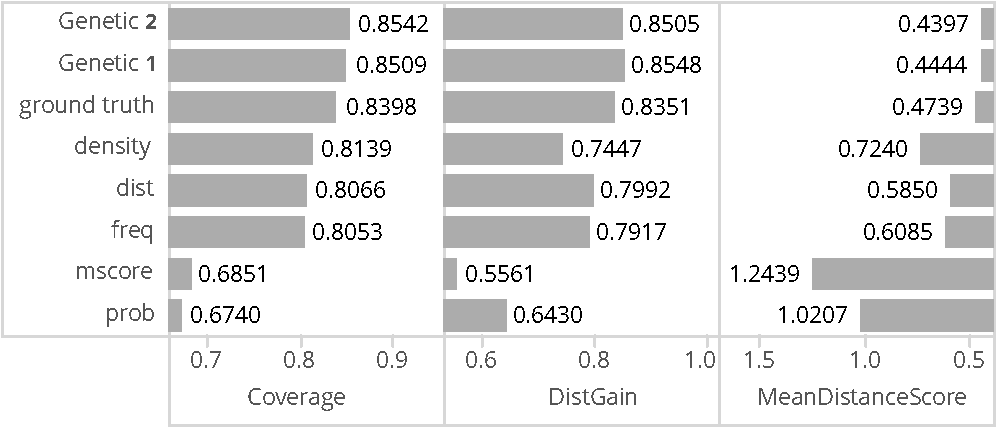
\includegraphics[width=0.7\columnwidth]{05_schema/eval_internal.pdf}
  \caption{Internal evaluation. The $Genetic_2$ has the best coverage and mean distance while $Genetic_1$ has the best distance gain.}
  \label{fig:eval_internal}
\end{figure}


\begin{wrapfigure}{l}{0.45\textwidth}
  \begin{center}
    \raisebox{0pt}[\dimexpr\height-3\baselineskip\relax]{\
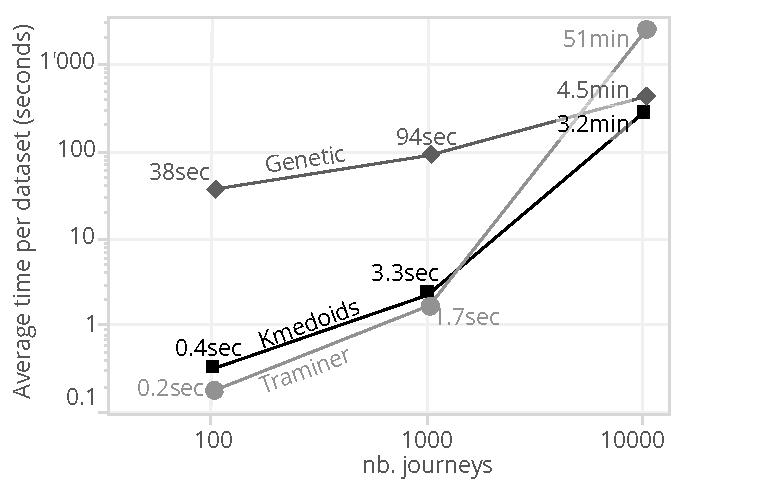
\includegraphics[width=0.42\columnwidth]{05_schema/time.pdf}
    }
  \end{center}
  \vspace{-20pt}
  \caption{Comparing the execution time per dataset for 100, 1'000, and 10'000 journeys.}
  \vspace{-20pt}
  \label{fig:performance-time}
\end{wrapfigure} 

Finally, the execution time to for 1,000 actual journeys is much faster using the approach with the techniques implemented in Traminer \cite{gabadinho2013searching} compared to our genetic approach. We compare how the different algorithms scale when the number of journeys increases. Hence, we ran each configuration five times with the 40 different datasets. Fig.~\ref{fig:performance-time} summarizes the results. As can be seen, the algorithms implemented in Traminer are orders of magnitude faster than our approach when dealing with 100 or 1,000 journeys. However, note that our algorithm has a better scaling potential when the number of journeys grows. All the algorithms tested tend to be slow and will not scale when dealing with several thousand journeys. 

\section{Experiments Using Real Datasets}

This section reports on the experiments with a real dataset, the goal being to illustrate how a change in the settings impacts the results.  We used a publicly available dataset\footnote{http://www.cmap.illinois.gov/data/transportation/travel-survey
} describing the activities performed throughout the day by Chicago's citizens. There are 15 types of activities, such as, `being at home', `attending class', `going shopping', or `doing households errands'. In the context of this dataset, a journey is the sequence of activities starting from the morning until the night. Typically, `being at home' $\rightarrow$ `attending class' $\rightarrow$ `being at home' is a journey consisting of three activities. The total number of journeys is 29,541 and there are 123,706 activities (with an average of 4.817 activities per journey). This dataset is interesting not only for the relatively large number of data points describing life trajectories, but also because of the available detailed contextual data, such as information on the citizens' demographics. 


\begin{wrapfigure}{r}{0.5\textwidth}
  \begin{center}
    \raisebox{-15pt}[\dimexpr\height-3\baselineskip\relax]{\
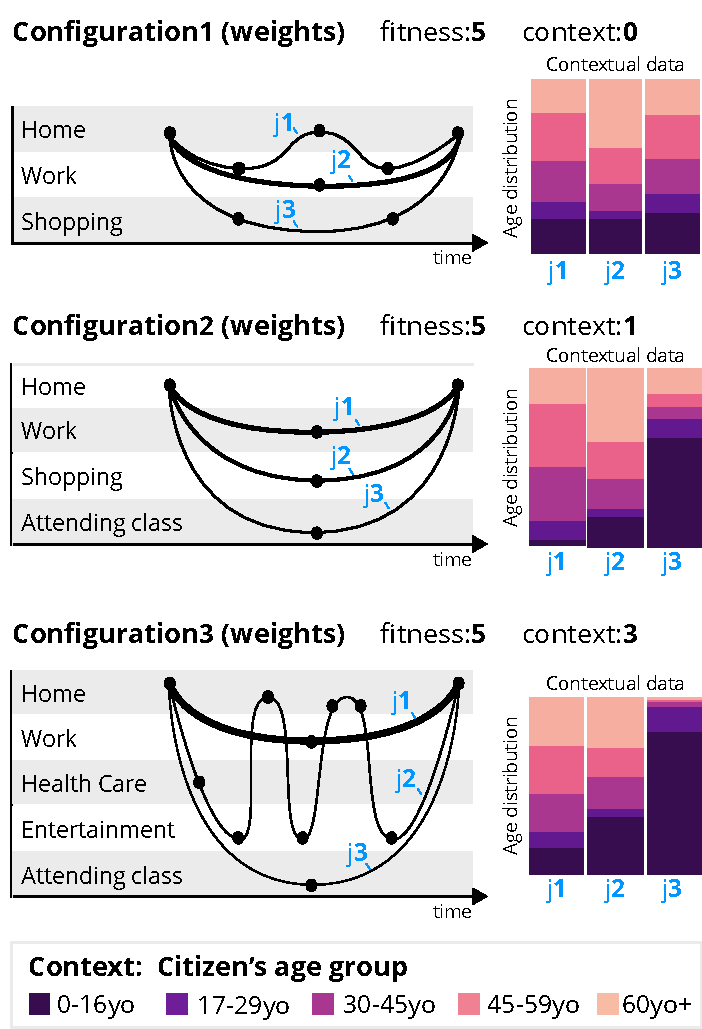
\includegraphics[width=0.48\columnwidth]{05_schema/results_real_dataset.pdf}
    }
  \end{center}
  \vspace{0pt}
  \caption{Results with real dataset using three configurations}
  \vspace{-10pt}
  \label{fig:results_real_dataset}
\end{wrapfigure} 

The goal of the experience is to show the influence of taking the citizen's age in consideration when measuring the distance between journeys. Fig.~\ref{fig:results_real_dataset} shows the results using three different configurations. In configuration 1, we did not leverage the contextual data (i.e., the contextual distance weight is set to 0). We interpret the resulting  CJM as follows. The first journey represents people going to `work', going back `home' at noon, and returning to `work' in the afternoon. The second journey is close to the first one, the main difference being that people do not seem to go back `home' at noon. The third journey shows citizens being at `home', going `shopping' twice in the afternoon, and going back `home'. 

In configuration 2, we test the effect on the resulting CJM when considering the ages of the customers. Therefore, we changed the weight put on the contextual distance from 0 to 1. As can be seen in Fig.~\ref{fig:results_real_dataset}, three representative journeys were generated. Each of these journeys has three touchpoints. They start from `home' and finish at `home'. In between, the first journey has the activity `work', the second one has the activity `shopping', and the last one the activity `attending class'. It is interesting to note the effect of the configuration on the contextual data (the distribution charts on the right side of Fig.~\ref{fig:results_real_dataset}). Indeed, while the age was equally distributed for each journey in configuration 1, we can observe that the age is discriminant in configuration 2. For instance, more than half of the citizens in the journey $j_3$ are under 16 years old, while this population represents only 8.7\% of the entire dataset.

In configuration 3, we show the effect when we increase the weight put on the contextual distance parameter. Journeys $j_1$ and $j_3$ are identical to those in configuration 2. However, a new and rather complex journey $j_2$ emerges. We observe that the distribution is impacted when giving more weight to homogeneity. We interpret the result as follows: Citizens younger than 29 years old tend to have two typical patterns of activities involving either `school' or `entertainment' while the most typical journeys for the other citizens involve `work'. 

Of course, this is an extremely simplified overview of the data. For the almost 30,000 actual journeys in the event logs, there are numerous unique actual journeys that differ from the representative journeys we get from these three configurations. By letting the user choose the weight for each parameter, we let them explore different perspectives of the data. We claim that the best parameters depend on the dataset, the business context, and the goal of the exploration. 


\section{Conclusion}
Our genetic approach to summarizing a set of customer journeys with the purpose of displaying them on a CJM offers an interesting alternative to approaches used in social sciences for three reasons. First, the quality of the results is better, which is true using both internal and external evaluation metrics. Second, the weights of the three quality criteria are a flexible way to analyze a dataset under different perspectives. All the other parameters, such as the number of representative journeys to display or the length of the representative journeys are left entirely to the genetic algorithm. Third, in addition to the sequence of activities, our genetic algorithm can leverage contextual data to group similar journeys. By doing so, we provide a way to summarize insights from customers that are hidden in the data. 

We tackle the task of building a CJM from event logs as a single-objective optimization problem so that a single `best' CJM is returned. Due to the inherent conflicting objectives of the quality criteria, we acknowledge that a multi-objective approach might be a relevant choice that we did not investigate.  

We show that techniques from social sciences are also useful for studying customer trajectories. As suggested by Gabadinho et al., ``The methods are by no way limited to social science data and should prove useful in many other domains'' \cite{gabadinho2009summarizing}. This present study supports this claim and highlights how research from social science can benefit our understanding of customers. At a time when a customer-centric culture has become important \cite{verhoef2009customer}, or even a matter of survival according to \cite{McKinsey2017cultureDig}, we anticipate that research at the crossroads between data science, marketing, and social sciences will be key to a full understanding of customer experiences. 


\bibliographystyle{splncs04}
\bibliography{bibliography.bib}


\end{document}
